\documentclass[a4paper, 12pt]{article}
\usepackage[margin=2.5cm]{geometry}
\usepackage[swedish]{babel}
\usepackage[T1]{fontenc}
\usepackage[utf8]{inputenc}
\usepackage{mathtools}
\usepackage{graphicx}
\usepackage{hyperref}
\usepackage{url}
\usepackage{array}
\usepackage[dvipsnames]{xcolor}
\usepackage{csquotes}
\usepackage{cite}
\usepackage{tikz}
\usepackage{subcaption}

\begin{document}

\begin{titlepage}
    % Uppsala logotyp
    \begin{tikzpicture}[remember picture, overlay]
        \node [anchor=north west, inner sep=30pt]  at (current page.north west)
            {
\includegraphics[height=4cm]{logo_uu_se.png}};
    \end{tikzpicture}

    \begin{center}
        % Rubrik
        {\LARGE \textbf{Nationskompassen} \\ \large Pubrundor för studenter i Uppsala} \\[2cm]

        % Nationskompassen logotyp
        \includegraphics[height=10cm]{logo_nationskompassen_utantext.png} \\[1cm]

        % Författare och handledare
        \textbf{Projektgrupp 50} \\
        Anton Äng \\
        Alexander Brundin \\
        Emil Reimegård \\[0.5cm]
        Handledare: Matilda Blomqvist \\

        % Datum
        \today

        % Kursinformation
        \vfill
        Projektrapport för kursen Programkonstruktion och datastrukturer \\
        Uppsala Universitet \\
        VT 26
    \end{center}
\end{titlepage}

\newpage

\tableofcontents

\newpage
% Introduktion
\section{Introduktion}
    Uppsala som studentstad präglas av dess nationer och de aktiviteter som med nationerna kommer till. Nationsguiden \cite{Nationsguiden} är en webbplats som samlar in och tillhandahåller information om de olika nationerna i Uppsala, inklusive deras evenemang, öppettider och kontaktinformation. Denna webbplats är avsedd att hjälpa både nya och befintliga studenter att navigera i det rika utbudet av nationer i Uppsala. Detta arbete menar dock att webbplatsen saknar viss funktionalitet. Möjligheten att kombinera nationers aktiviteter och evenemang är något som Nationsguiden inte själva implementerat, det initiativet står istället användaren för och kan vara tidskrävande. Nationskompassen som program ses kunna komplettera denna brist i funktionalitet hos Nationsguiden, i hopp om att öka användarvänligheten för studenter på Uppsala Universitet.


    Nationskompassen är ett program som utnyttjar den information som Nationsguiden tillhandahåller för att skapa den kortaste pubrundan möjlig utifrån de nationspubbar som för ett givet datum är öppna, vart användaren vill påbörja sin pubrunda samt hur många nationspubbar som rundan ska innehålla. Genom detta erbjuder Nationskompassen en effektiv lösning på att slå samman nationers evenemang och planera pubrundor.

% Guide
\section{Guide till Nationskompassen}
\label{sec: guide}

    Det här avsnittet beskriver hur du installerar och använder Nationskompassen steg för steg, från installation till en färdig pubrunda.

    \subsection{Förutsättningar}

        Innan du kan köra Nationskompassen behöver följande vara installerat på din dator:

        \begin{itemize}
            \item \textbf{Node.js} (version 18 eller senare) -- används för att köra TypeScript-projekt.
            \item \textbf{npm} -- pakethanterare som följer med Node.js.
            \item \textbf{ts-node} -- används för att köra \texttt{.ts}-filer direkt utan att kompilera dem manuellt.
        \end{itemize}

        Kontrollera att Node.js och npm är installerade genom att köra följande kommandon i terminalen (se \hyperref[fig:guide-versions]{Figur~\ref*{fig:guide-versions}}).

    \subsection{Installation}

        \begin{enumerate}
            \item Ladda ner eller klona projektmappen till din dator.
            \item Navigera till projektets rotmapp i terminalen.
            \item Installera projektets beroenden med \texttt{npm} (se \hyperref[fig:guide-npm-install]{Figur~\ref*{fig:guide-npm-install}}).
        \end{enumerate}

        Projektets mappstruktur bör se ut ungefär som i \hyperref[fig:guide-folder-structure]{Figur~\ref*{fig:guide-folder-structure}}.

    \subsection{Starta programmet}

        Kompilera \texttt{main.ts}, se \hyperref[fig:guide-compile]{Figur~\ref*{fig:guide-compile}}. Kör programmet från projektets rotmapp med kommandot \texttt{node main.js} (se \hyperref[fig:guide-start-cmd]{Figur~\ref*{fig:guide-start-cmd}}).
        När programmet startar hämtas aktuell data från nationsguiden.se och du möts av startmenyn (se \hyperref[fig:guide-main-menu]{Figur~\ref*{fig:guide-main-menu}}).

    \subsection{Visa öppna pubbar}

        Välj alternativ \textbf{2} för att se en lista över alla nationspubbar som är öppna just nu. För varje pub visas organisation, pubnamn, kontaktinformation och öppettider (se \hyperref[fig:guide-open-pubs]{Figur~\ref*{fig:guide-open-pubs}}).

    \subsection{Skapa en pubrunda}

        Välj alternativ \textbf{1} för att skapa en pubrunda. Programmet visar de tillgängliga pubarna numrerade och ber dig välja en startpub och hur många stopp du vill göra.

        \subsubsection*{Steg 1 -- Välj startpub}

        En numrerad lista visas med alla öppna pubbar. Ange numret för den pub du vill börja på (se \hyperref[fig:guide-choose-start]{Figur~\ref*{fig:guide-choose-start}} och \hyperref[fig:guide-startpub-exempel]{Figur~\ref*{fig:guide-startpub-exempel}}).

        \subsubsection*{Steg 2 -- Välj antal stopp}

        Ange hur många pubbar du vill besöka totalt under rundan (se \hyperref[fig:guide-choose-stops]{Figur~\ref*{fig:guide-choose-stops}}).

        \subsubsection*{Steg 3 -- Din färdiga pubrunda}

        Programmet beräknar den kortaste möjliga rundan och presenterar resultatet (se \hyperref[fig:guide-finished-route]{Figur~\ref*{fig:guide-finished-route}}). Ordningen på pubarna är beräknad geografiskt, så att du alltid tar det kortast möjliga steget till nästa pub. Du kan skapa hur många rundor som helst under samma session.

    \subsection{Avsluta programmet}

        Skriv \textbf{Q} (eller \textbf{q}) i huvudmenyn för att avsluta programmet (se \hyperref[fig:guide-quit]{Figur~\ref*{fig:guide-quit}}).

    \subsection{Felhantering och vanliga problem}

        \begin{itemize}
            \item \textbf{Inga pubbar visas:} Det kan bero på att inga nationer har öppet det aktuella datumet, eller att nonce-värdet i \texttt{collect\_data.ts} behöver uppdateras. Se avsnitt \hyperref[subsec: svagheter]{\textit{5.2 Svagheter}} för mer information.
            \item \textbf{Ogiltigt val i menyn:} Om du anger ett tal utanför det giltiga intervallet i startmenyn, uppmanar programmet dig att försöka igen (se \hyperref[fig:guide-invalid-input]{Figur~\ref*{fig:guide-invalid-input}}).
            \item \textbf{Färre stopp än önskat:} Om du begär fler stopp än det finns öppna pubbar avslutas rundan i förtid med ett meddelande (se \hyperref[fig:guide-too-few-pubs]{Figur~\ref*{fig:guide-too-few-pubs}}).
        \end{itemize}

% Dokumentation
\section{Programdokumentation}
\label{sec: dokumentation}

    \subsection{Allmän design på programmet}
    \label{subsec: design}
        Nationskompassen är en pubrundsplanerare för Uppsalas studentnationer. Den låter användaren välja startpub och längden på rutten. Därefter hämtar den data från hemsidan nationsguiden.se och genererar den geografiskt sett kortaste pubrundan baserat på användarens val. Programmet Nationskompassen är uppdelat i sex moduler med olika ansvarsområden:
        \begin{itemize}
            \item \textbf{\texttt{collect\_data}} - Hämtar information från nationsguiden.se
            \item \textbf{\texttt{extract\_essential\_data}} - Extraherar relevant information från collect\_data
            \item \textbf{\texttt{build\_nation\_matrix}} - Använder relevant information för att konstruera en viktad graf
            \item \textbf{\texttt{create\_route}} - Skapar en pubrunda utifrån en viktad graf
            \item \textbf{\texttt{user\_input}} - Möjliggör för användaren att interagera med programmet
            \item \textbf{\texttt{main}} - Den drivande modulen som koordinerar de andra modulerna
        \end{itemize}
        Strukturen i programmet är sekventiell. Under \hyperref[subsec: flöde]{\textit{3.5 Kontrollflöde och hjälpfunktioner}} finns det en mer djupgående förklaring på hur programmets olika moduler samspelar samt en grafisk visualisering. 

    \subsection{Viktiga datastrukturer och algoritmer}
    \label{subsec: DSAL}

        \subsubsection{Datastrukturer}
        \label{subsubsec: DS}
            \paragraph{NationNode}
                är den centrala datastrukturen i programmet. Varje nationspub representeras som en NationNode. Den innehåller organisationsnamn, pubnamn, öppetider, kontaktinformation, geografiska koordinater samt nationens vikt som används vid avståndsberäkningar.

            \paragraph{NationMatrix}
                är en tvådimensionell array av NationNodes som fungerar som en viktad matris. Raden $i$ och kolumnen $j$ håller en kopia av NationNode$(j)$ där vikten är satt till avståndet mellan nation$(i)$ och nation$(j)$. Diagonalelementen, det vill säga en nations avstånd till sig själv, är alltid 0.

            \paragraph{NationIndex}
                är en Map av typ \texttt{\{string, number\}} som kopplar nationsnamnet till ett index $(i)$ i NationMatrix för att snabbt kunna slå upp ett nationsindex.

            \paragraph{Set$\langle$number$\rangle$}
                är ett set som håller redan besökta nationer för att säkerställa att samma nation inte besöks två gånger.
            
            \paragraph{Pair$\langle$string, number$\rangle$}
                används för att ta emot användarens val: startpub och antal nationer.

        \subsubsection{Algoritmer}
        \label{subsubsec: AL}
            Programmet använder två viktiga algoritmer som återfinns i \texttt{get\_distance} och \texttt{nearest\_nation}. \texttt{get\_distance} utnyttjar Pythagoras sats för att beräkna avståndet mellan två nationer med hjälp av deras latitud- och longitudkoordinater. \texttt{nearest\_nation} är en så kallad girig närmaste-granne-algoritm. Det innebär att den vid varje nytt steg under sökningen gör valet enbart baserat på vad som är bäst i stunden. I \texttt{nearest\_nation} innebär det att den alltid väljer den nation som ligger närmast den nation den befinner sig på just nu.

    \subsection{Moduler och bibliotek}
    \label{subsec: modul_och_bib}
        Nationskompassen importerar två bibliotek: \texttt{nation.ts} samt \texttt{list.ts}. \texttt{list}-biblioteket är taget från det bibliotek kursen tillhandahåller och därifrån hämtas typen \texttt{Pair} och konstruktorfunktionen \texttt{pair}, som används för att representera användarens val som ett par av startnation och antal stopp. Dessutom hämtas välj-funktionerna \texttt{head()} samt \texttt{tail()}. \texttt{nation}-biblioteket innehåller alla relevanta typer för programmet, beskrivna i avsnitt \hyperref[subsec: DSAL]{\textit{3.2 Viktiga datastrukturer och algoritmer}}, samt en statisk array som håller koordinaterna till alla nationer. Modulen \texttt{readline} har använts för att möjliggöra inläsning av indata från användaren i terminalen.

    \subsection{Viktiga funktioner}
    \label{subsec: viktiga_func}
        \begin{itemize}
            \item \texttt{main()} är startpunkten för hela programmet. Anropar relevanta funktioner för datainsamling och bearbetning samt hanterar eventuella fel med try/catch.
            \item \texttt{get\_events()} skickar ett anrop till nationsguiden.se och returnerar en array av typen \texttt{NationGuideCategory}.
            \item \texttt{get\_open\_pubs()} filtrerar en array av typen \texttt{NationGuideCategory[]} baserat på event som tillhör kategorin ''Pub'' och returnerar en array med \texttt{NationGuideEvent}.
            \item \texttt{extract\_essentials()} omvandlar en array av typen \texttt{{}NationGuideEvent[]} till en array av \texttt{NationNode} genom att extrahera relevant information från varje instans av \texttt{NationGuideEvent}. Använder hjälpfunktionen \texttt{get\_organiser\_coordinates()} för att hämta nationens koordinater från koordinatarrayen i nationsbiblioteket. Returnerar en array av \texttt{NationNode}.
            \item \texttt{build\_nation\_distance\_matrix()} bygger en viktad tvådimensionell matris av typen \texttt{NationMatrix} baserat på en array av \texttt{NationNode}. Bestämmer vikten med hjälp av \texttt{get\_distance()} som beräknar avståndet mellan två nationer med hjälp av Pythagoras sats.
            \item \texttt{build\_nation\_index()} kopplar varje nationnamn till ett index med den inbyggda Map-funktionen. Används för att snabbt slå upp ett nationsindex.
            \item \texttt{nearest\_nation()} hittar den närmaste, ej besökta nationen som inte är den nuvarande. Returnerar den närmast tillgängliga nationen.
            \item \texttt{create\_route()} tar emot användarens val av startnation samt antal pubar som önskas besökas. Skapar pubrundan med hjälp av repetitiva anrop till \texttt{nearest\_nation()} tills pubrundan uppfyller användarens krav eller tills det inte finns fler pubar att besöka.
        \end{itemize}

    \subsection{Kontrollflöde och hjälpfunktioner}
    \label{subsec: flöde}

        Programmet börjar i \texttt{main()}, som koordinerar samtliga anrop under programmets körning. Det första steget är att hämta data, vilket sker genom ett anrop till \texttt{get\_events()}. Den funktionen utför ett anrop till nationsguiden.se och returnerar rådata som en array av \texttt{NationGuideCategory}.


        Rådata skickas vidare till \texttt{get\_open\_pubs()}, som filtrerar bort alla evenemang som inte tillhör kategorin ''Pub'' och returnerar en array av typen \texttt{NationGuideEvent}. Denna array skickas i sin tur till \texttt{extract\_essentials()}, som omvandlar varje enskilda event till en \texttt{NationNode}. För att göra detta anropar \texttt{extract\_essentials()} sin privata hjälpfunktion \texttt{get\_organiser\_coordinates()}, vilken slår upp nationens GPS-koordinater i den statiska koordinatarrayen som återfinns i nationsbiblioteket. Koordinaterna läggs sedan in i \texttt{NationNode}-objektet.


        Den resulterande arrayen av \texttt{NationNode} skickas slutligen till \texttt{create\_route()} tillsammans med användarens val av startnation och antal stopp. Inuti \texttt{create\_route()} sker en intern kedja av anrop: först byggs distansmatrisen upp via \texttt{build\_nation\_distance\_matrix()}, som internt anropar sin hjälpfunktion \texttt{get\_distance()} för att beräkna det relativa avståndet mellan varje nation och dess grannar. Därefter anropas \texttt{build\_nation\_index()} för att kunna slå upp startnationers index i matrisen. Sedan itererar \texttt{create\_route()} och anropar \texttt{nearest\_nation()} upprepade gånger tills pubrundan uppfyller det antal stopp som användaren angett eller tills dess att inga fler tillgängliga nationer finns.


        Hjälpfunktionen \texttt{get\_organiser\_coordinates()} är privat, funktionen är definierad inuti sin föräldrarfunktion och anropas aldrig direkt utifrån. Den används enbart för att hålla föräldrarfunktionens logik läsbar och välstrukturerad. Hjälpfunktionen \texttt{get\_distance()} är global, men anropas enbart av \texttt{build\_nation\_distance\_matrix()}. Anledningen till detta är att kunna exportera funktionen enskilt, vilket möjliggör testning av avståndslogik.


        Slutligen returnerar \texttt{create\_route()} den färdiga pubrundan som en array av strängar, vilket \texttt{main()} skriver ut i terminalen. För en grafisk representation av dataflödet, se \hyperref[fig:dataflöde]{Figur~\ref*{fig:dataflöde}}, notera att det som presenteras i figuren endast innefattar datahantering. Kopplingen mellan användare och Nationskompassen enkapsuleras istället av modulerna \texttt{main} och \texttt{user\_input}.

\section{Testning}
    Testning är en central del av mjukvaruutveckling som syftar till att säkerställa en programvaras pålitlighet, funktionalitet och kvalitet. Som en del av detta projektarbete och utvecklingen av Nationskompassen använts testning för att verifiera att de olika komponenterna i programmet fungerar och samverkar som tänkt. Eftersom den data som tillhandahålls av nationsguiden.se kan variera, är det avgörande att programmet kan hantera dessa variationer korrekt. Testningen utfördes på två nivåer: enhetstestning och integrationstestning. Enhetstestning fokuserade på att testa individuella funktioner och moduler i isolering, medan integrationstestningen syftade till att säkerställa huruvida data flödar genom programmets olika komponenter som tänkt. Testningen utfördes med Jest (ett enkelt JavaScript-testramverk \cite{jest}.). All testning genomfördes med syntetisk data och är uppdelad i tre delar, en del för modulen \texttt{extract\_essential\_data}, en för \texttt{build\_nation\_matrix} och slutligen en för \texttt{create\_route}. För en överblick på testernas resultat, se \hyperref[fig: jest_results]{Figur~\ref*{fig: jest_results}}.

    \subsection{\texttt{extract\_essential\_data}}
    \label{subsec: extract_essential_data}
        Här testades funktionerna \texttt{get\_open\_pubs()} och \texttt{extract\_essentials()}. Testerna täcker olika scenarion, inklusive fall där det inte finns några öppna pubar, fall där det finns flera öppna pubar och fall där data innehåller oväntade format eller saknade fält. Testerna verifierar att \texttt{get\_open\_pubs()} korrekt filtrerar ut endast de evenemang som tillhör kategorin ''Pub'' och att \texttt{extract\_essentials()} korrekt extraherar och omvandlar informationen till \texttt{NationNode}-objekt. Därefter utfördes även tester på särskilda/få förekommande scenarion, såsom de fall där data innehåller oväntade format eller där viss data förekommer i dubbletter. Samtliga testningar för Nationskompassen följer liknande struktur, därav agerar \hyperref[fig: overview_tests]{Figur~\ref*{fig: overview_tests}} exempel för en överblick på en moduls tester och \hyperref[fig: example_tests]{Figur~\ref*{fig: example_tests}} exempel för hur ett tester kan se ut.

    \subsection{\texttt{build\_nation\_matrix}}
    \label{subsec: build_nation_matrix}
        I denna del av testningen säkerställdes att skapandet av en \texttt{NationMatrix} var korrek genom funktionerna \texttt{get\_distance()}, \texttt{build\_nation\_index()} samt \texttt{build\_nation\_distance\_matrix()}. Testerna säkerställde bland annat att \texttt{get\_distance()} korrekt beräknar de relativa avståndet mellan två \texttt{NationNode}, att \texttt{build\_nation\_index()} korrekt tillger en \texttt{NationNode} ett index och att \texttt{build\_nation\_distance\_matrix()} returnerar en pålitlig struktur av en \texttt{NationMatrix}. Därefter säkerställdes även att funktionerna fungerade som tänkt i ett integrationstest, där en \texttt{NationMatrix} skapades och vardera \texttt{NationNode} tilldelades ett giltigt index.

    \subsection{\texttt{create\_route}}
    \label{subsec: create_route}
        I sista steget av testningen säkerställdes att skapandet av pubrundan var pålitlig genom funktionerna \texttt{nearest\_nation()} samt \texttt{create\_route()}. Testerna verifierade exempelvis att en pubrunda inte innehöll dubbletter av nationer och att pubrundans längd var anpassad både efter efterfrågan men också antalet tillgängliga nationspubbar.

\section{Diskussion}
\label{sec: diskussion}
    \subsection{Val under projektets gång}
    \label{subsec: val}
        Projektet inleddes med en vision där användaren skulle använda programmet i ett grafiskt användargränssnitt. Flera olika tekniker diskuterades innan det fastställdes att HTML skulle användas för att representera data grafiskt. Denna vision ändrades dock tidigt under projektets gång och istället för ett grafiskt användargränssnitt så exekveras programmet direkt i terminalen. Anledningen till detta var främst tidsbrist, men även att den grafiska delen inte var en del av kursens lärandemål.


        Ett annat val som gjordes tidigt in i projektet var huruvida data som skulle användas var riktig data eller om den skulle ha varit syntetisk data. Det beslutades om att använda riktig data som hämtades från Nationsguiden, detta för att det skulle vara mer realistiskt och för att det skulle vara mer intressant att arbeta med riktig data. Detta ledde fram till nästa problem, hur skulle data hämtas? 


        Där togs beslutet att huvudfokuset med projektet är inte att implementera en form of web scraper, utan mer att hantera den inhämtade data. Därför valdes att använda en AI-assistent för att generera funktionen som hämtar data från Nationsguiden och parsar den till ett format som enklare kan hanteras.

        
        Det sista stora beslutet som togs var att övergå från den ursprungliga visionen av att programmet skulle spara data för varje nation i hashtabeller, till att istället representera nationerna som noder i en viktad graf. För att sedan med hjälp av en grafalgoritm hitta den kortaste vägen mellan noderna. Detta beslut togs eftersom relationerna mellan nationerna bättre kan beskrivas som ett nätverk. En graf gör det möjligt att representera nationerna som noder och avstånden mellan dem som vikter på kanterna. 

    \subsection{Svagheter}
    \label{subsec: svagheter}
        Programmets främsta svaghet finns redan innan inhämtningen av data, för att hämta data så måste funktionen uppdateras med ett nonce-värde, en sträng med nummer som uppdateras två gånger under dagen som hämtas från Nationsguiden. I denna version av Nationskompassen saknas giltig kontaktinformation till varje nation, istället har det fältet för varje nation fyllts med \texttt{[N\textbackslash A, N\textbackslash A]}.

    \subsection{Framtida projekt}
    \label{subsec: framtid}
        Hade det funnits mer tid så hade det varit intressant att få implementera det grafiska användargränssnittet som nämndes ovan. Det hade bidragit till användarupplevelsen och gjort det mer tillgängligt för användare som inte är bekväma med att använda terminalen.


        Det hade också varit bra att hitta en metod så nonce-värdet inte behöver uppdateras manuellt varje gång data ska hämtas. Det diskuterades olika idéer för att lösa detta. Bland annat genom att använda det TypeScript-kompatibla verktyget Playwright, som hade kunnat användas för att spela in stegen som behövs för att hämta nonce-värdet. För att därefter köra den delen av programmet innan data hämtas.

        Som nämnts ovan under \hyperref[subsec: svagheter]{\textit{5.2 Svagheter}} saknar vardera nation giltig kontaktinformation. Programmet har därför konstruerats modulärt, där kontaktinformationen lagras i ett separat fält för varje nation. Detta gör det möjligt att komplettera med korrekt information i ett senare skede utan att påverka övriga delar av systemet.

        Det hade även varit intressant att implementera funktionalitet som exempelvis möjlighet att spara sina rutter, haft en mobilanpassning, ge förslag på slutdestinationer utefter andra evenemang, storlek på sällskap, m.m. 

\section{Sammanfattning}
\label{sec: sammanfattning}
Nationskompassen är ett terminalbaserat program som hjälper studenter i Uppsala att planera pubrundor bland stadens nationer. Programmet hämtar realtidsdata från nationsguiden.se och genererar, utifrån användarens val av startpub och antal stopp, den geografiskt kortaste möjliga pubrundan med hjälp av en girig närmaste-granne-algoritm över en viktad graf.

Programmet är uppdelat i sex moduler med tydliga ansvarsområden, från datainsamling och bearbetning till ruttgenerering och användarinteraktion. Testning genomfördes med Jest på enhetsnivå och integrationsnivå för att säkerställa programmets tillförlitlighet.

Projektet resulterade i ett fungerande program som uppfyller sitt syfte, men har identifierade svagheter -- framför allt kravet på manuell uppdatering av ett nonce-värde vid datahämtning. Framtida förbättringar skulle kunna inkludera ett grafiskt användargränssnitt, automatiserad datahämtning samt utökad funktionalitet som sparade rutter och mobilanpassning.

\newpage
\bibliographystyle{plain}
\bibliography{referenser}
\newpage
\appendix
\section*{Bilagor}
\label{sec: bilagor}
\addcontentsline{toc}{section}{Bilagor}
\begin{figure}[htbp]
    \centering
    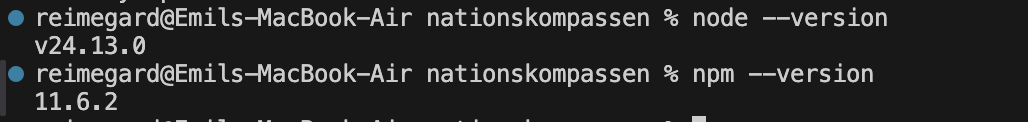
\includegraphics[width=\linewidth]{./guide_bilder/version_control.png}
    \caption{Kontroll av Node.js- och npm-version i terminalen.}
    \phantomsection
    \label{fig:guide-versions}
\end{figure}

\begin{figure}[htbp]
    \centering
    
\includegraphics[width=\linewidth]{./guide_bilder/npm_install.png}
    \caption{Körning av \texttt{npm install} i projektmappen.}
    \phantomsection
    \label{fig:guide-npm-install}
\end{figure}

\begin{figure}[htbp]
    \centering
    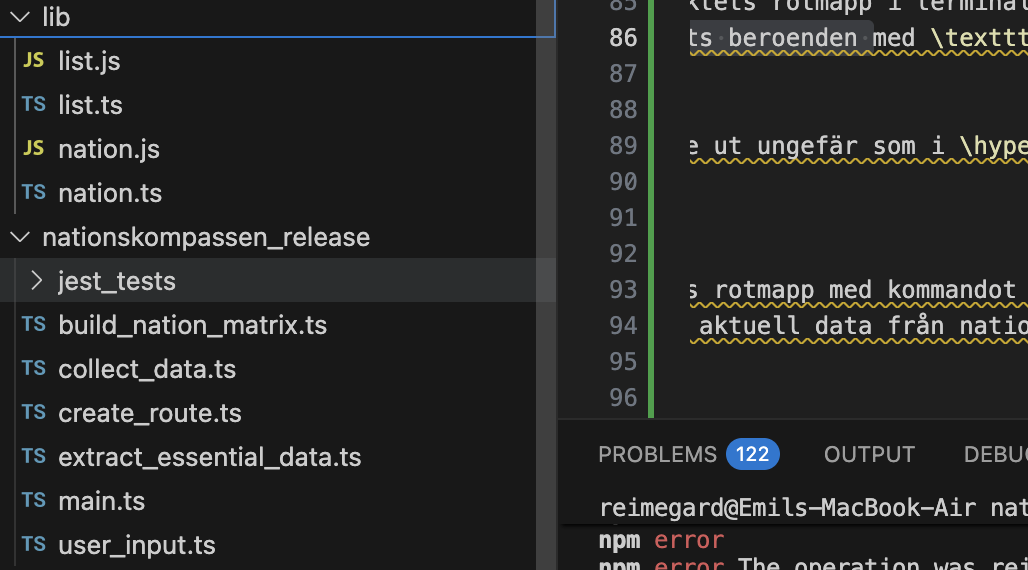
\includegraphics[width=0.6\linewidth]{./guide_bilder/struktur.png}
    \caption{Projektets mappstruktur i VS Code.}
    \phantomsection
    \label{fig:guide-folder-structure}
\end{figure}

\begin{figure}[htbp]
    \centering
    
\includegraphics[width=\linewidth]{./guide_bilder/kompilera.png}
    \caption{Kompilering av projektet med \texttt{tsc main.ts}.}
    \phantomsection
    \label{fig:guide-compile}
\end{figure}

\begin{figure}[htbp]
    \centering
    
\includegraphics[width=\linewidth]{./guide_bilder/start.png}
    \caption{Startkommando \texttt{node main.js} i terminalen.}
    \phantomsection
    \label{fig:guide-start-cmd}
\end{figure}

\begin{figure}[htbp]
    \centering
    
\includegraphics[width=\linewidth]{./guide_bilder/Startmeny.png}
    \caption{Startmenyn i Nationskompassen.}
    \phantomsection
    \label{fig:guide-main-menu}
\end{figure}

\begin{figure}[htbp]
    \centering
    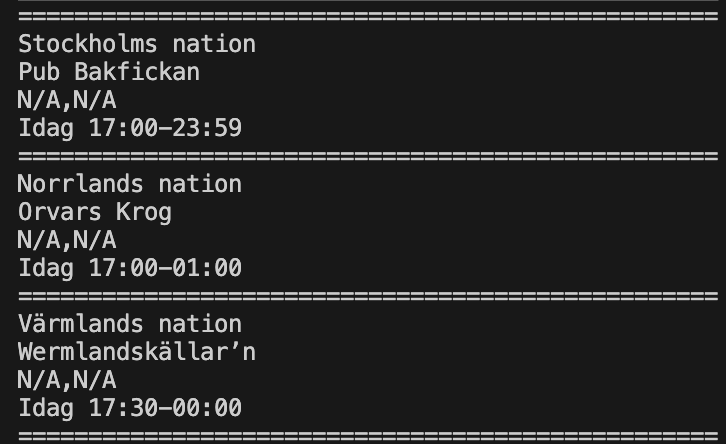
\includegraphics[width=\linewidth]{./guide_bilder/visa_pubar.png}
    \caption{Lista över öppna nationspubbar (alternativ 2).}
    \phantomsection
    \label{fig:guide-open-pubs}
\end{figure}

\begin{figure}[htbp]
    \centering
    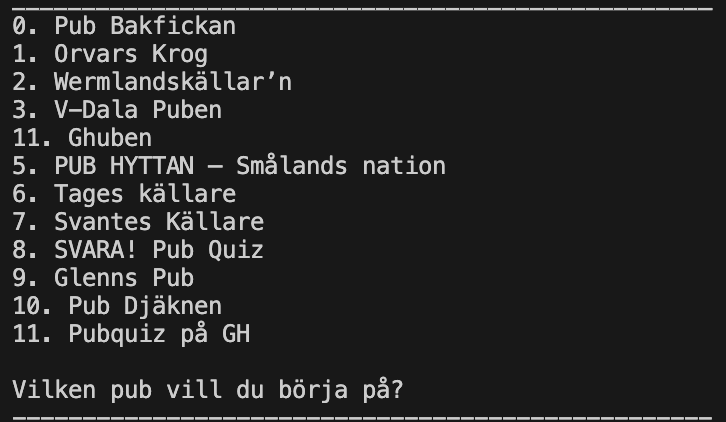
\includegraphics[width=\linewidth]{./guide_bilder/valja_startpub.png}
    \caption{Val av startpub -- numrerad lista över tillgängliga pubbar.}
    \phantomsection
    \label{fig:guide-choose-start}
\end{figure}

\begin{figure}[htbp]
    \centering
    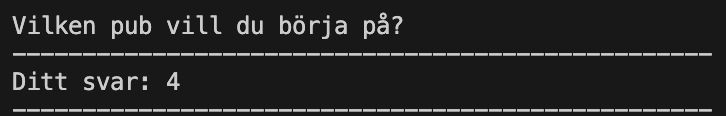
\includegraphics[width=\linewidth]{./guide_bilder/startpub_exempel.png}
    \caption{Exempel på inmatat svar vid val av startpub.}
    \phantomsection
    \label{fig:guide-startpub-exempel}
\end{figure}

\begin{figure}[htbp]
    \centering
    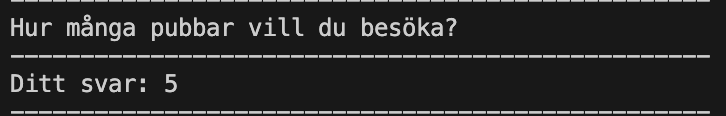
\includegraphics[width=\linewidth]{./guide_bilder/langd_exempel.png}
    \caption{Val av antal stopp i pubrundan.}
    \phantomsection
    \label{fig:guide-choose-stops}
\end{figure}

\begin{figure}[htbp]
    \centering
    
\includegraphics[width=\linewidth]{./guide_bilder/fardig_runda.png}
    \caption{Den färdiga pubrundan presenteras i terminalen.}
    \phantomsection
    \label{fig:guide-finished-route}
\end{figure}

\begin{figure}[htbp]
    \centering
    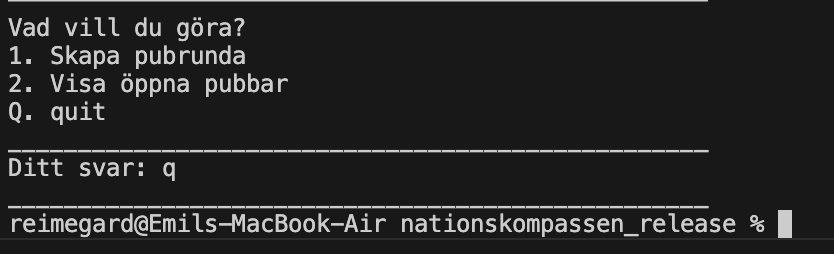
\includegraphics[width=\linewidth]{./guide_bilder/quit.png}
    \caption{Avslutning av programmet med kommandot Q.}
    \phantomsection
    \label{fig:guide-quit}
\end{figure}

\begin{figure}[htbp]
    \centering
    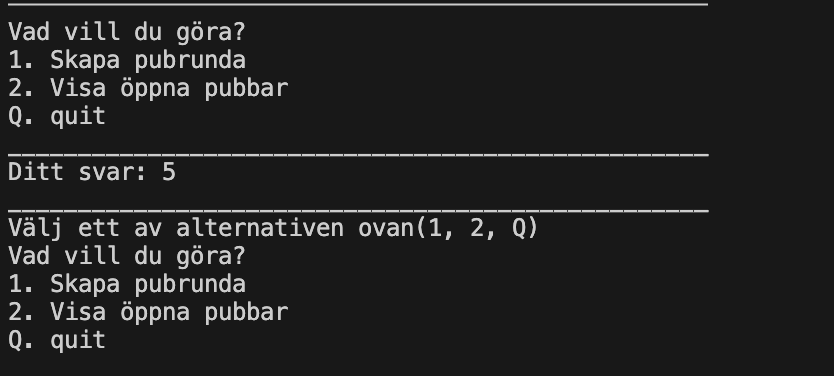
\includegraphics[width=\linewidth]{./guide_bilder/fel_input_meny.png}
    \caption{Felmeddelande vid ogiltigt menyval.}
    \phantomsection
    \label{fig:guide-invalid-input}
\end{figure}

\begin{figure}[htbp]
    \centering
    
\includegraphics[width=\linewidth]{./guide_bilder/for_lang.png}
    \caption{Meddelande när önskat antal stopp överstiger tillgängliga pubbar.}
    \phantomsection
    \label{fig:guide-too-few-pubs}
\end{figure}

\begin{figure}[htbp]
    \centering
        
\includegraphics[width=\linewidth]{projekt_backend.jpg}
        \caption{Flödeschema för hur data från nationsguiden.se flödar igenom Nationskompassen.}
        \phantomsection
        \label{fig:dataflöde}
\end{figure}

\begin{figure}[htbp]
    \centering

        \begin{subfigure}{0.5\textwidth}
            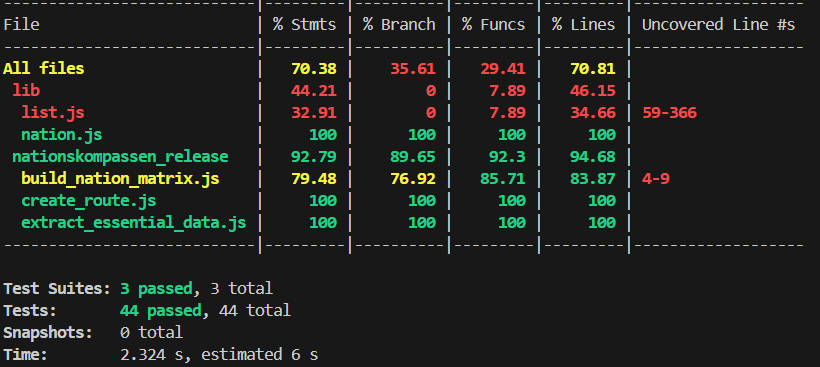
\includegraphics[width=\linewidth]{./jest_bilder/resultat_coverage.png}
            \caption{Samtliga test och andelen testad kod från vardera fil.}
        \end{subfigure}

        \begin{subfigure}{0.5\textwidth}
            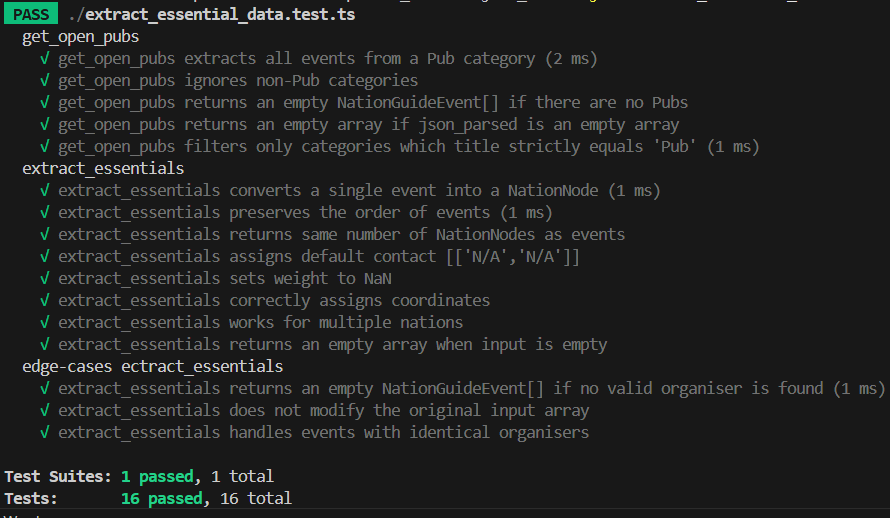
\includegraphics[width=\linewidth]{./jest_bilder/resultat_extract_essential_data.png}
            \caption{överblick på tester för \texttt{extract\_essential\_data}.}
        \end{subfigure}

        \begin{subfigure}{0.5\textwidth}
            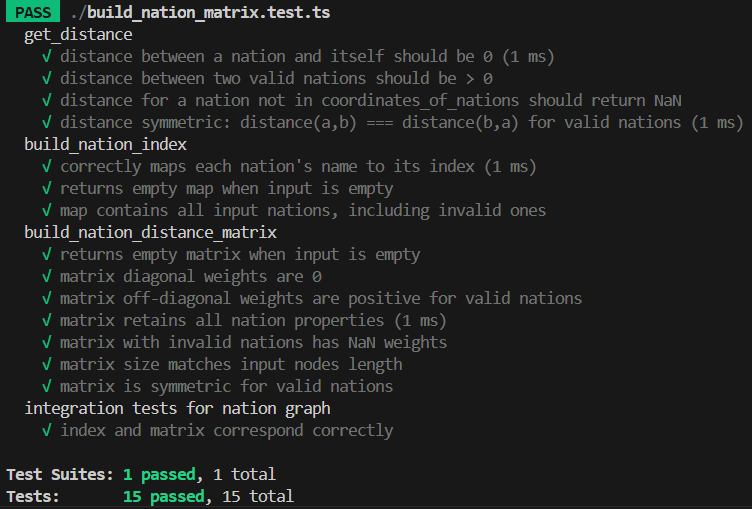
\includegraphics[width=\linewidth]{./jest_bilder/resultat_build_nation_matrix.png}
            \caption{Överblick på tester för \texttt{build\_nation\_matrix}.}
        \end{subfigure}

        \begin{subfigure}{0.5\textwidth}
            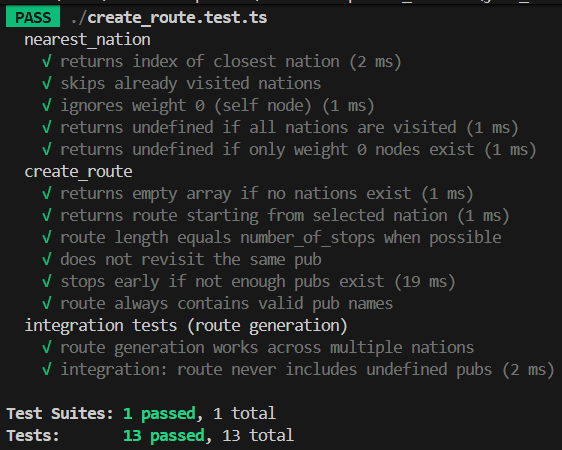
\includegraphics[width=\linewidth]{./jest_bilder/resultat_create_route.png}
            \caption{Överblick på tester för \texttt{create\_route}.}
        \end{subfigure}
        
        \caption{Överblick på resultaten från Jest-tester}
        \phantomsection
        \label{fig: jest_results}
\end{figure}

\begin{figure}[htbp]
    \centering

        \begin{subfigure}{0.6\textwidth}
            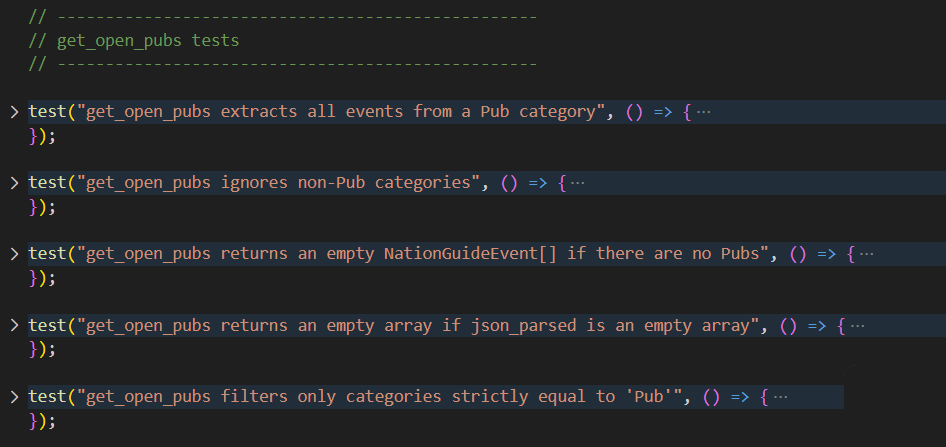
\includegraphics[width=\linewidth]{./jest_bilder/get_open_pubs.test.png}
            \caption{Tester för \texttt{get\_open\_pubs()}}
        \end{subfigure}

        \begin{subfigure}{0.6\textwidth}
            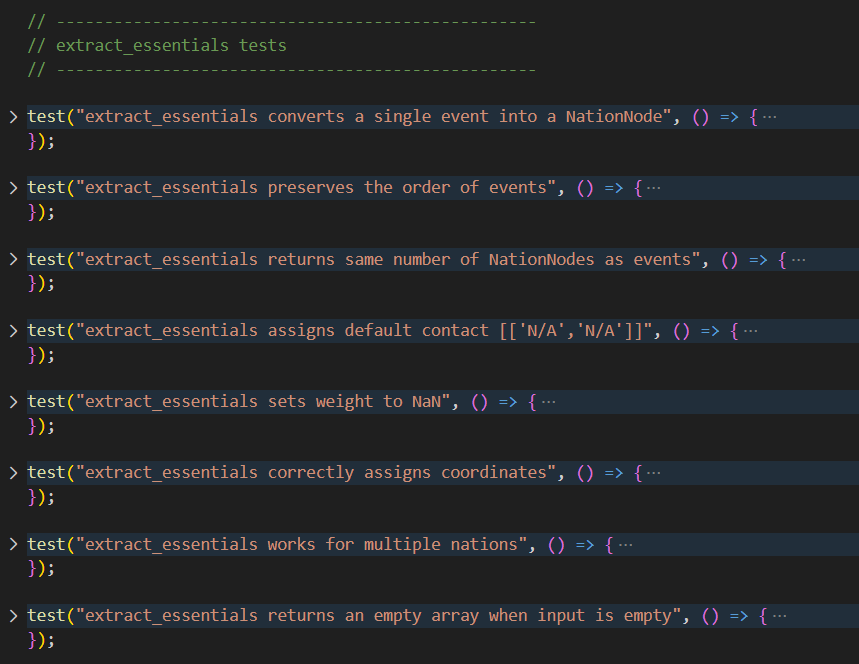
\includegraphics[width=\linewidth]{./jest_bilder/extract_essentials.test.png}
            \caption{Tester för \texttt{extract\_essentials()}}
        \end{subfigure}

        \begin{subfigure}{0.6\textwidth}
            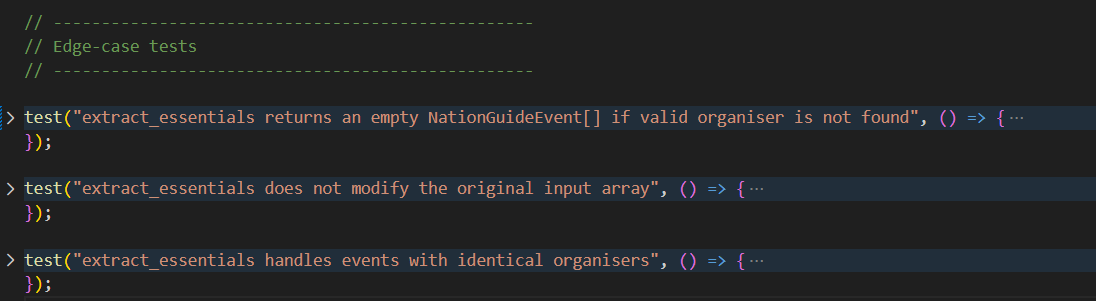
\includegraphics[width=\linewidth]{./jest_bilder/extract_essential_data_edge.test.png}
            \caption{Edge-case tester}
        \end{subfigure}

        \caption{Översikt av Jest-tester för modulen \texttt{extract\_essential\_data}.}
        \phantomsection
        \label{fig: overview_tests}
\end{figure}
\newpage
\begin{figure}[htbp]
    \centering

        \begin{subfigure}{0.7\textwidth}
            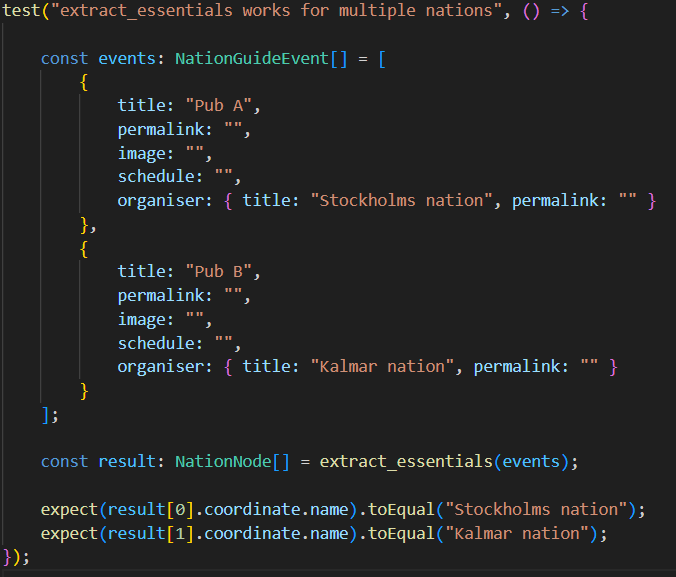
\includegraphics[width=\linewidth]{./jest_bilder/ex_test.png}
            \caption{Exempel på standardtest}
        \end{subfigure}

        \hfill

        \begin{subfigure}{0.7\textwidth}
            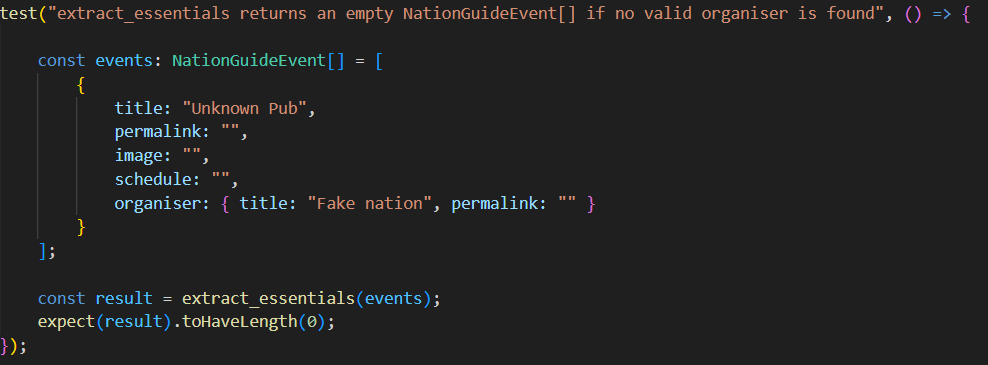
\includegraphics[width=\linewidth]{./jest_bilder/ex_test_edge.png}
            \caption{Exempel på edge-case test}
        \end{subfigure}
        
        \caption{Exempel på individuella Jest-tester för extraktionsfunktionerna.}
        \phantomsection
        \label{fig: example_tests}
\end{figure}

\end{document}